\subsection{\acrshort{pcb}}

Zu dieser Schaltung wurde auch ein \gls{pcb} entworfen.
Das \gls{pcb} ist sowohl in \autoref{fig:pcb}, als auch genauer unter \autoref{apx:pcb} in \autoref{fig:pcb-2d} und \autoref{fig:pcb-3d} dargestellt.
Der Schaltplan ist in \autoref{apx:schematic} inkludiert.
Auf dem Board ist ein \texttt{555} Timer zur \gls{pwm} Erzeugung und zwei \texttt{LM75B} Sensoren verbaut.
Die beiden Sensoren sind dem \texttt{TMP102} sehr ähnlich, sind jedoch vorrätig.
Deren Adressen werden jedoch durch die Addresspins verändert.
Der \texttt{OS} Pin der beiden Sensoren wird auch angeschlossen.
Da dieser in Open-Drain Konfiguration benutzt werden kann, belegen beide Signale nur einen Pin.
Momentan wird der Übertemperaturalarm nicht in der Software benutzt.
Die Änderungen ab Treiber für die \texttt{LM75B} Sensoren ist trivial.
Momentan besteht keine Softwareunterstützung für zwei Sensoren, jedoch ist diese Modifikation trivial.
Das \gls{pcb} ist \gls{rpi} \textit{HAT} konform und respektiert mechanische und elektronische Anforderungen\footnote{Diese Anforderungen spezifizieren beispielsweise den mechanischen Umriss, die nicht-leitenden Befestigungslöcher und die Belegung der 40-Pin Steckverbindung.}.

\begin{figure}[h]
    \centering
    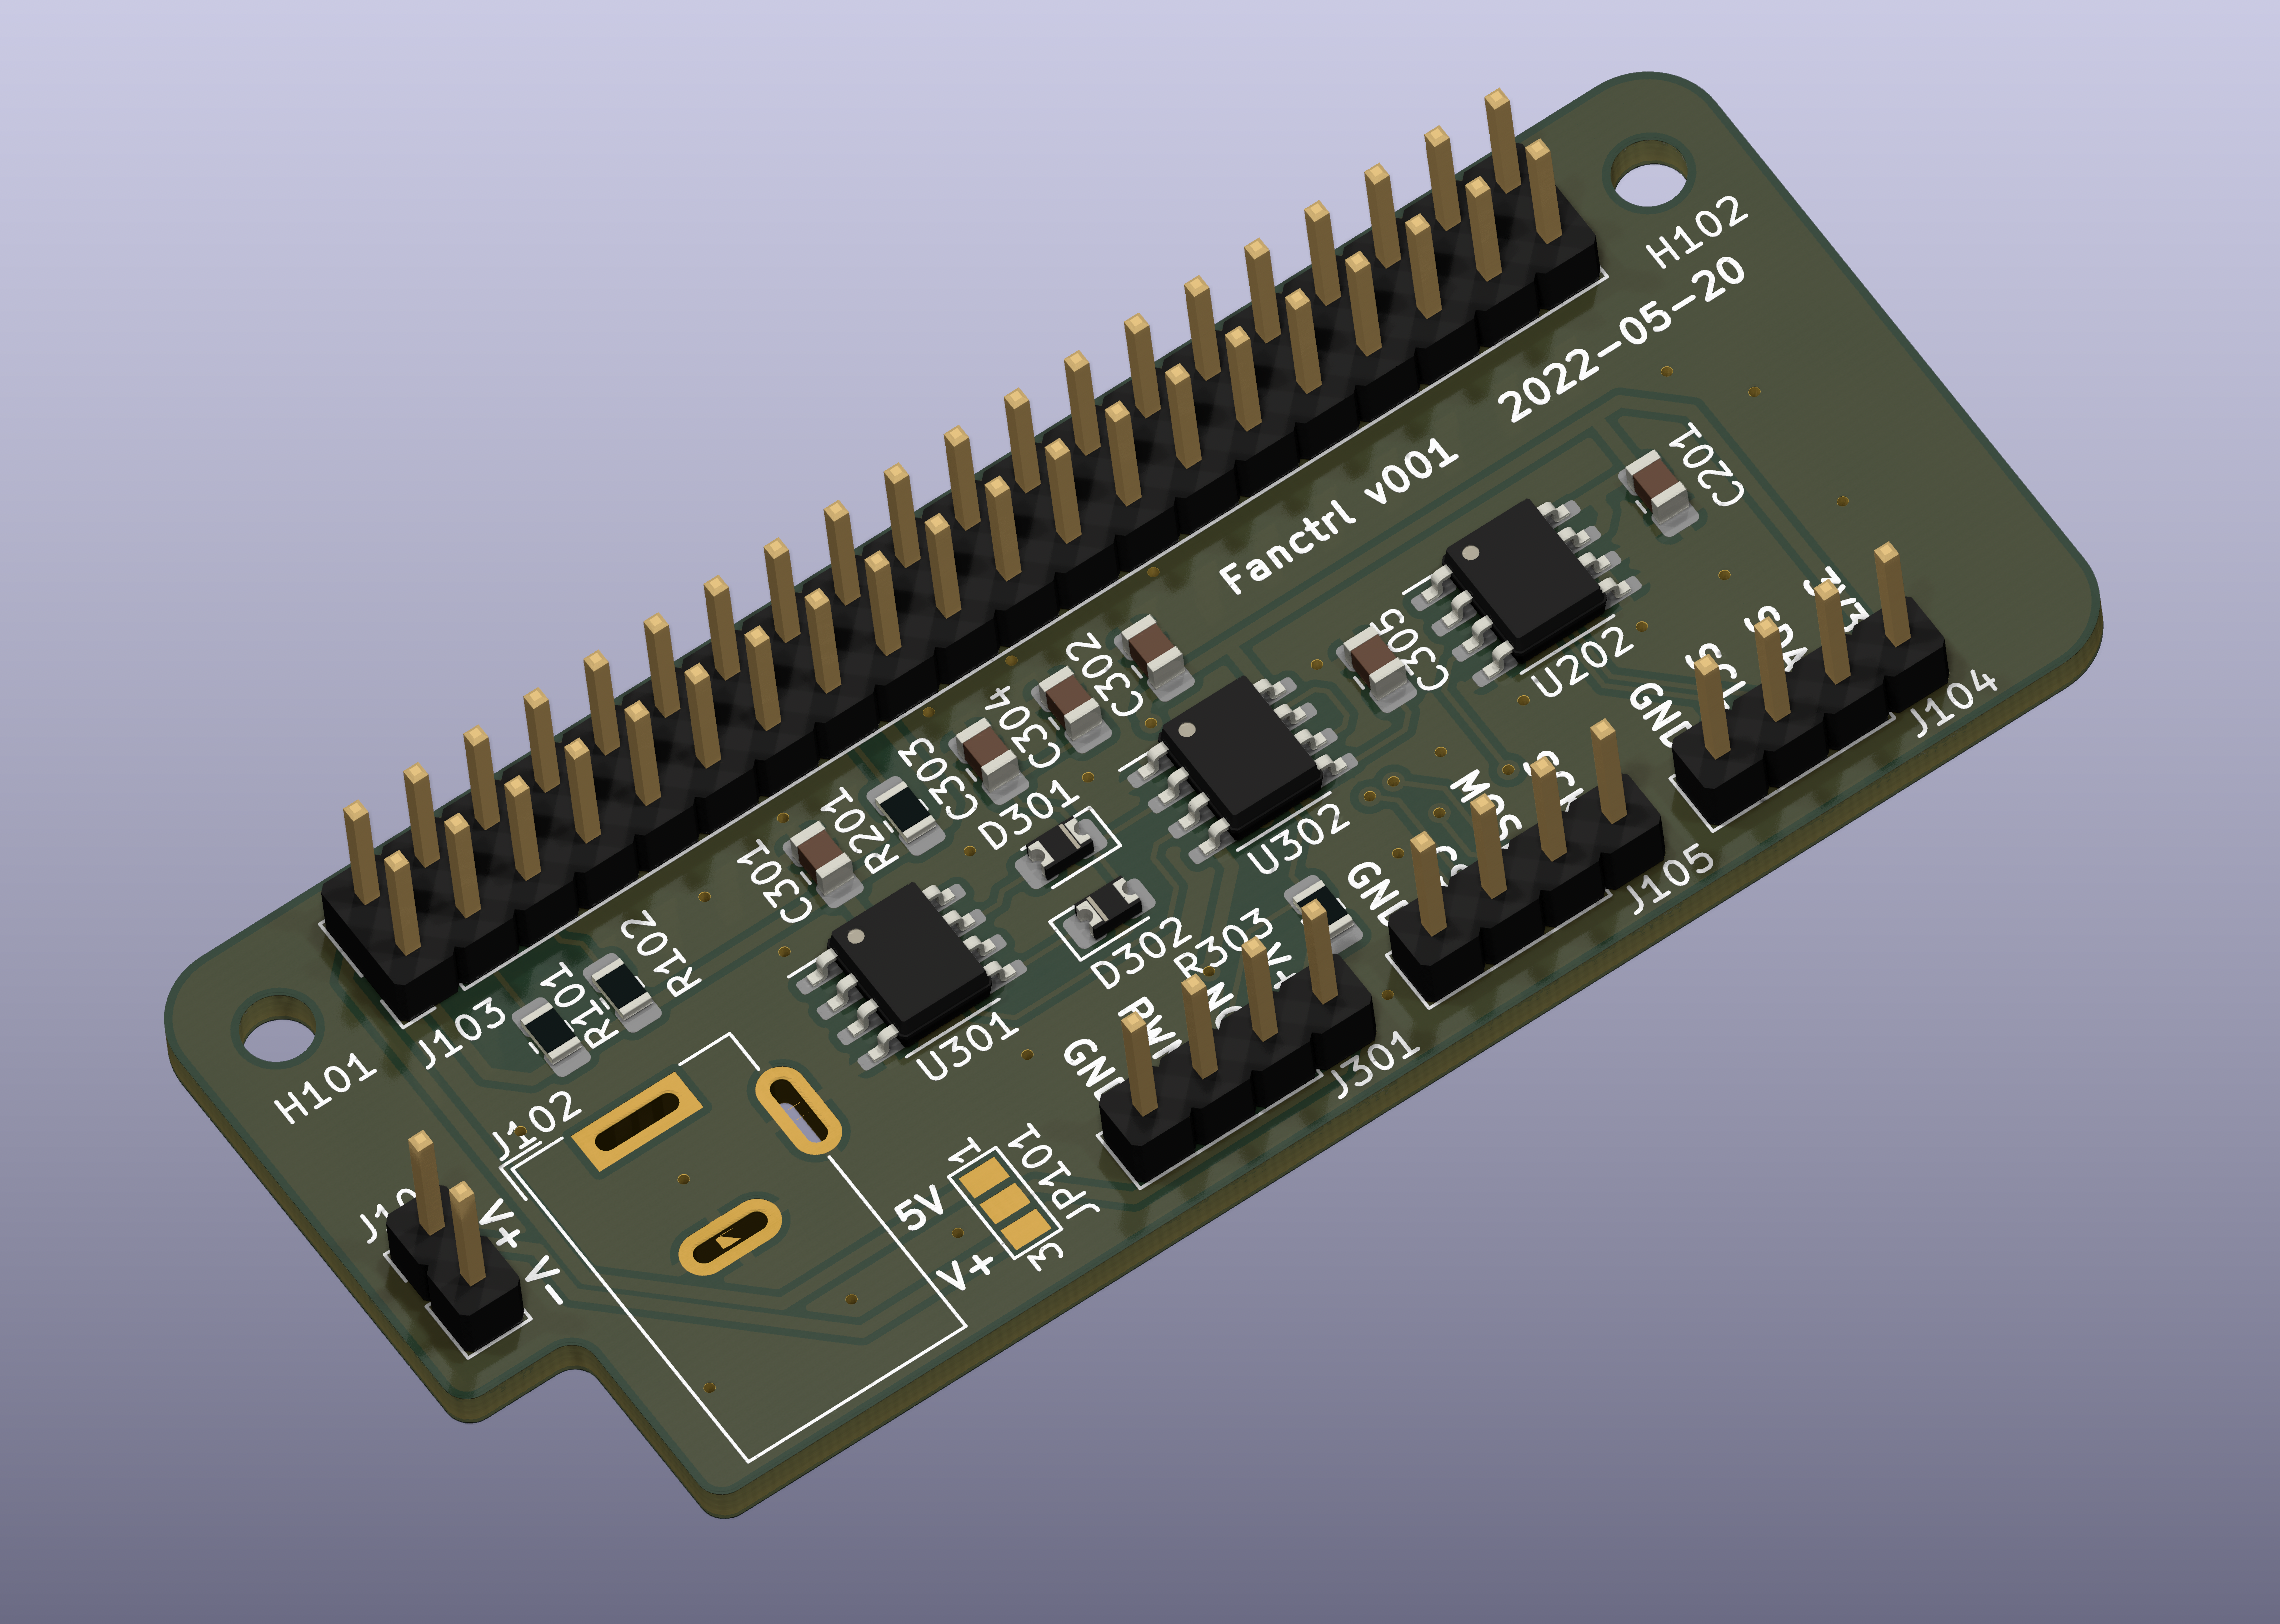
\includegraphics[width=9cm]{./img/pcb-3d-top.png}
    \caption{TOP-Seite des entworfenen \gls{pcb}}
    \label{fig:pcb}
\end{figure}
